\chapter*{Progetto}
\addcontentsline{toc}{chapter}{Progetto} % add the chapter to the index
Ad affiancare questa relazione è stata realizzata una demo implementativa che è possibile provare navigando all'indirizzo \url{https://tendto.github.io/EW-showcase/}.
Al fine di visionare tutte le funzioni, è necessario dotarsi dell'estensione browser \href{https://metamask.io/}{MetaMask}, \href{https://energyweb.atlassian.net/wiki/spaces/EWF/pages/703201459/Volta+Connecting+to+Remote+RPC+and+Metamask}{connettersi alla rete Volta} e avere a disposizione qualche \href{https://voltafaucet.energyweb.org/}{Volta token}. \\

La \gls{dapp}, che rappresenta la sintesi del progetto, ha come scopo quello di mostrare in azione le funzionalità \gls{ewns} (\autoref{sec:ewns}), \gls{did} (\autoref{sec:did}) e \gls{iam} (\autoref{sec:iam}), utilizzando, ove possibile, le librerie e i frameworks messi a disposizione da \gls{ew}.

\begin{figure}[h]
    \centering
    \subfloat[\centering \gls{did}]{{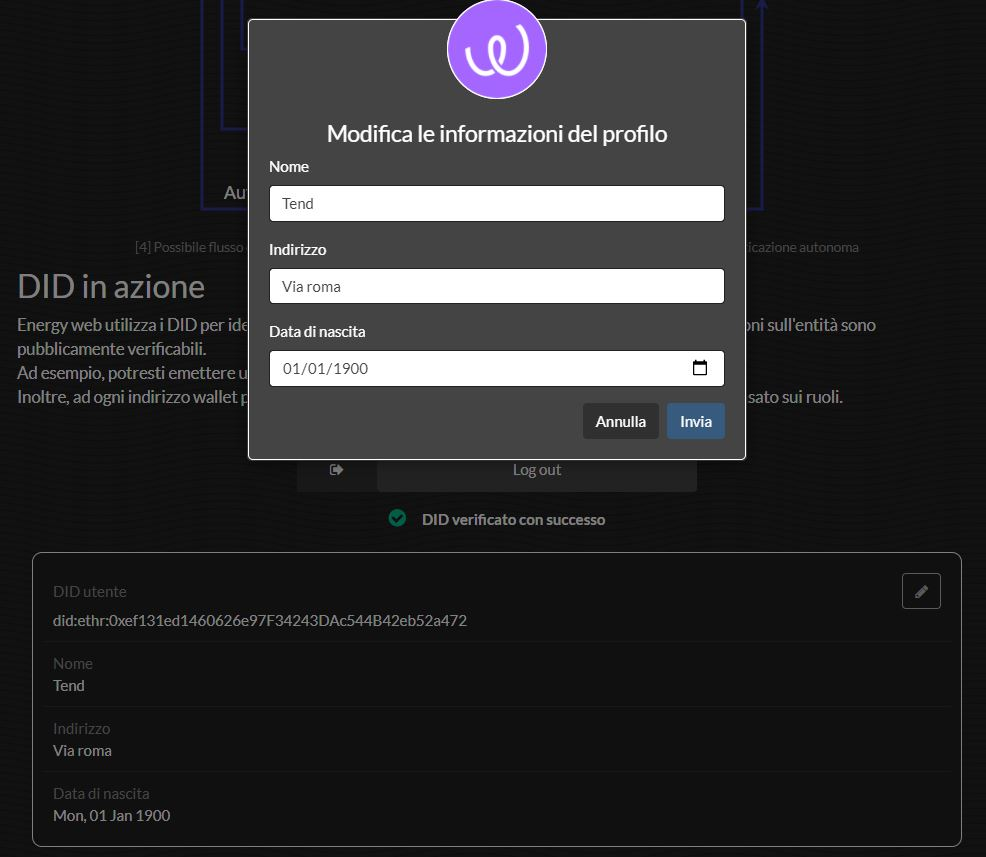
\includegraphics[width=6cm]{DID.jpg} }}
    \qquad
    \subfloat[\centering \gls{iam}]{{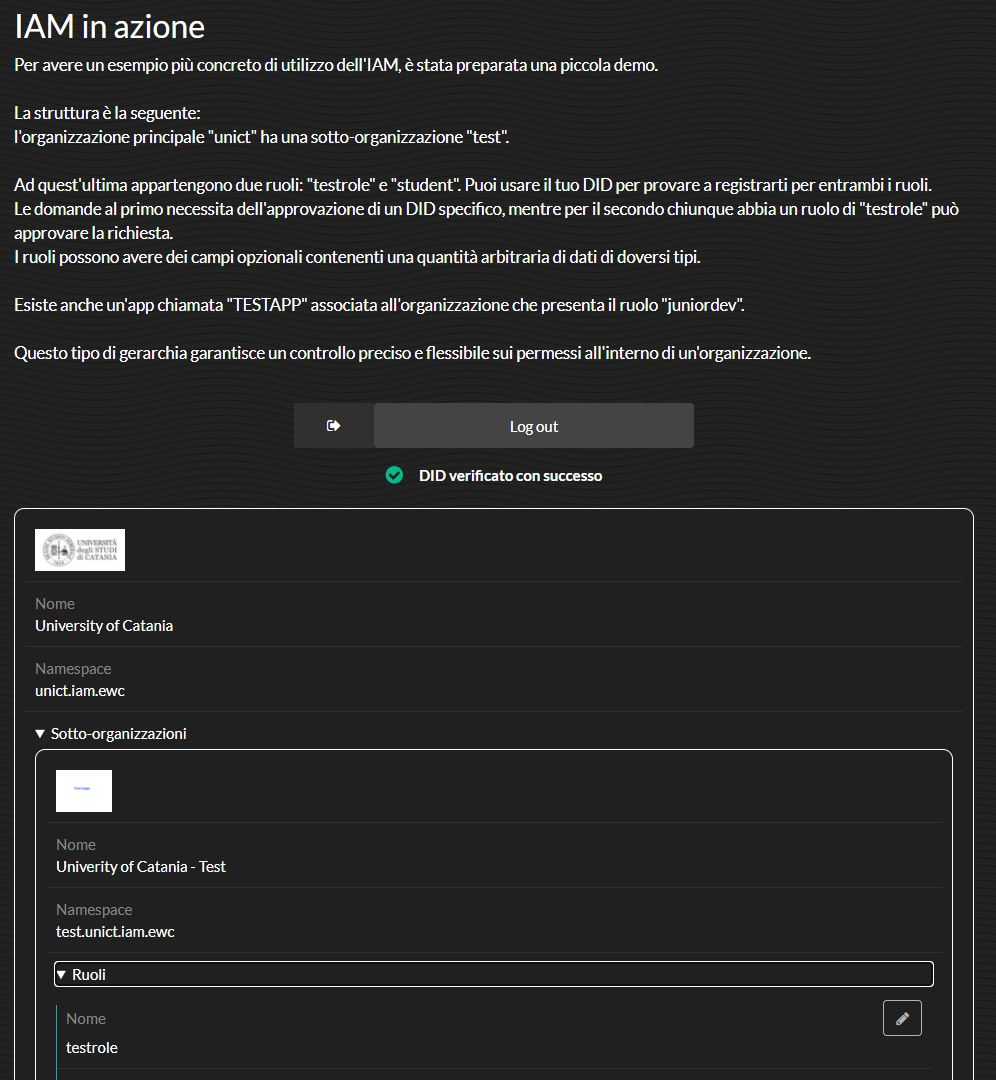
\includegraphics[width=6cm]{IAM.jpg} }}
    \caption{Screenshots della \gls{dapp}}
    \label{lab:project}
\end{figure}

L'intera documentazione e il codice dell'implementazione sono disponibili nella repository pubblica \href{https://github.com/TendTo/EW-showcase}{EW showcase} (\url{https://github.com/TendTo/EW-showcase}) su Github.